\FloatBarrier
\section{IAdapter}

IAdapter is a JMeter Plugin to perform evolutionary load, performance or stress tests. JMeter is a desktop application, designed to test and measure the performance and functional behavior of applications \cite{Nevedrov2007}. The IAdapter plugin implements the solution proposed in the section 6

The JMeter have components organized  in a hierarchical manner. The IAdapter plugin provides three main components: WorkLoadThreadGroup, WorkLoadSaver, and WorkLoadController.
 
The WorkLoadThreadGroup is a component that creates an initial population and configure the algorithms used in IAdapter . The Fig. \ref{fig:tela1iadapter} presents the main screen of the WorkLoadThreadGroup component. The component has a name \ding{202}, a set of configuration tabs \ding{203}, a list of individuals by generation \ding{204}, a button to generate an initial population \ding{205} and a button to export the results \ding{206}.

\begin{figure}[h]
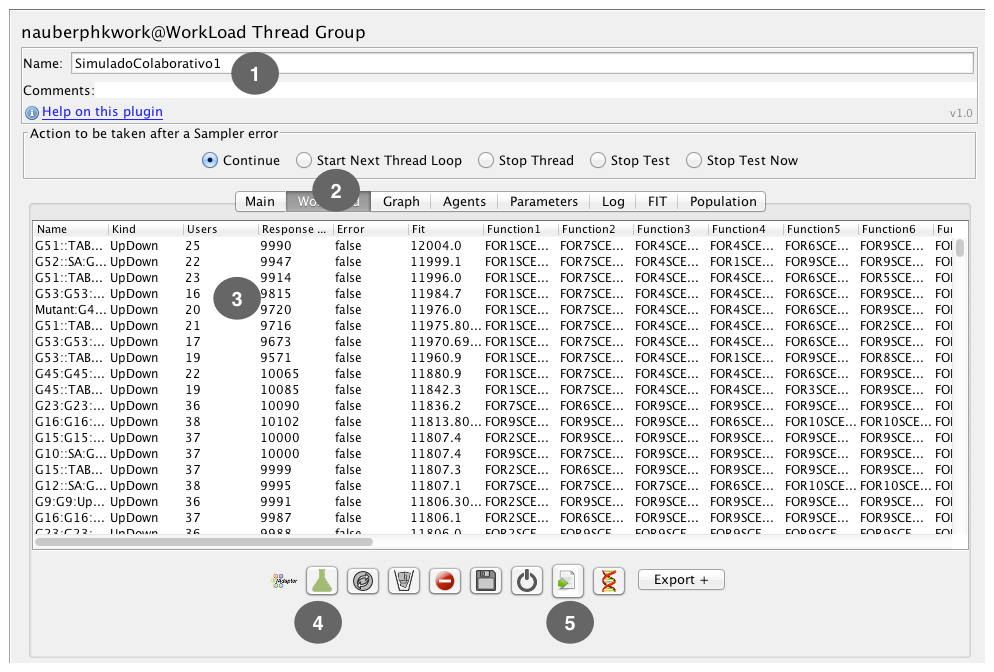
\includegraphics[width=0.5\textwidth]{./images/tela1iadapter.png}
\caption{WorkLoadThreadGroup component}
\label{fig:tela1iadapter}
\end{figure}

The WorkLoadSaver component is responsible for saving all data in the database. The operation of the component only requires its inclusion in the test script.

The WorkLoadController represents a scenario of test. The WorkLoadController represents a scenario of test. All actions necessary to test a application should be included in this component. All instance of the component need to login in the application under test and return the application to it's original state.

